\documentclass[
  letterpaper,
  twocolumn,
  9pt,
  journal,
  final]{IEEEtran}

\usepackage[spanish,es-tabla]{babel}
\usepackage[utf8]{inputenc}
\usepackage{amsfonts}
\usepackage{amsmath}
\usepackage{amssymb}
\usepackage{amsxtra}
\usepackage{mathrsfs}
\usepackage{array}
\usepackage{cite}
\usepackage{varioref}
\usepackage{float}
\usepackage{color}
\usepackage{colortbl}
\usepackage{enumerate}
\usepackage{rotating}
\usepackage{subcaption}
\usepackage{hyperref}
\usepackage{listings}
\usepackage{lipsum}
%\usepackage{flushend}
\usepackage{graphicx}


\title{Tarea 3 - Procesamiento Digital de Imágenes}
\author{\textbf{Autor:} Pablo Yáñez Santibáñez - pablo.yanez@uai.cl}
%\author{\IEEEauthorblockN{Pablo Yáñez S.} - pablo.yanez@uai.cl}

% Levels to show in table of contents:
% \setcounter{tocdepth}{-1} % only parts
% \setcounter{tocdepth}{0}  % only parts and chapters
% \setcounter{tocdepth}{1}  % part,chapters,sections
% \setcounter{tocdepth}{2}  % part,chapters,sections, subsections
% \setcounter{tocdepth}{3}  % part,chapters,sections, subsections,subsubsections
% \setcounter{tocdepth}{4}  % part,chapters,sections, subsections,subsubsections and paragraphs
% \setcounter{tocdepth}{5}  % part,chapters,sections, subsections, subsubsections, paragraphs and subparagraphs.


\begin{document}
\bstctlcite{IEEEexample:BSTcontrol}
\maketitle

% \begin{abstract}
% We propose \lipsum[1]
% \end{abstract}

\tableofcontents

% \listoffigures

% \listoftables

%%%%%%%%%%%%%%%%%%%%%%%%%%%%%%%%%%%%%%%%%%%%%%%%%%%%%%%%%%%%%%%%%%%%%%%%%%%%%%%%
\section{Marco Teórico}

En el procesamiento de de señales si bien es posible realizar operaciones en el dominio del tiempo o es espacio, este tipo de operaciones tienen una alta complejidad en terminos computacionales. Una alternativa para sobrellevar esto es aplicar una transformación matemática para cambiar el dominio de trabajo de la señal. En el ámbito del procesamiento de señales se utiliza la tranformada de Fourier, que tiene como base la Serie de Fourier.

%%%%%%%%%%%%%%%%%%%%%%%%%%%%%%%%%%%%%%%%%%%%%%%%%%%%%%%%%%%%%%%%%%%%%%%%%%%%%%%%
\subsection{Series de Fourier - Señales Continuas}

Jean-Baptiste Joseph Fourier propuso a comienzos del Siglo XIX que cualquier función periódicas de periodo $T$ puede descomponerse en la suma infinita de funciones $sin()$ y $cos()$. La expansión en series de Fourier de una función $f(x)$ esta dada por la expresión \ref{eq:fs}, mientras que los terminos $a_0$, $a_n$ y $b_n$ se calculan segun \ref{eq:fs_a0}, \ref{eq:fs_an} y \ref{eq:fs_bn} respectivamente.




\begin{align}
	f(x) &= \frac{a_0}{2} + \sum_{n=1}^{\infty} a_n cos \left(\frac{2n\pi}{T}x\right) + \sum_{n=1}^{\infty} b_1 sin\left(\frac{2n\pi}{T}x\right) \label{eq:fs} \\
	a_0 &= \frac{1}{T} \int_{t_0}^{t_0 + T} f(x) dx \label{eq:fs_a0} \\
	a_n &= \frac{1}{T} \int_{t_0}^{t_0 + T} f(x) cos(nx) dx \label{eq:fs_an}\\
	b_n &= \frac{1}{T} \int_{t_0}^{t_0 + T} f(x) sin(nx) dx \label{eq:fs_bn}
\end{align}

Otra forma de expresar la expansion en series de Fourier de un función es utilizar la expresión en notación en exponencial, la cual se desprende al utilizar la identidad de Euler.

\begin{align}
	f(x) &= \sum_{-\infty}^{\infty} c_n e ^ {-i \frac{2\pi n}{T} x} \label{eq:fs_euler}\\
	c_N &= \frac{1}{T} \int_{t_0}^{t_0 + T} f(x) e ^ {-i \frac{2\pi n}{T} x} dx
\end{align}

Las expresiones \ref{eq:fs} y \ref{eq:fs_euler} son formas equivalentes de expresar la representación en series de Forier de una señal periodica y real.

%%%%%%%%%%%%%%%%%%%%%%%%%%%%%%%%%%%%%%%%%%%%%%%%%%%%%%%%%%%%%%%%%%%%%%%%%%%%%%%%
\subsection{Transformada de Fourier - Señales Continuas}

La transformada de Fourier corresponde a una generalización de la serie de Fourier para señales no periódicas.
Si se tiene una función no periódica $x(t)$ como la presentada en la Figura \ref{fig:senal_aperidica} es posible construir una nueva señal periodica $x_p(t)$ con periodo $T_p$ repitiendo esta señal. Luego, $x(t)$ es igual a $x_p(t)$ cuando $T_p \to \infty$.

\begin{figure}[h!]
\centering
	\begin{subfigure}[b]{\columnwidth}
	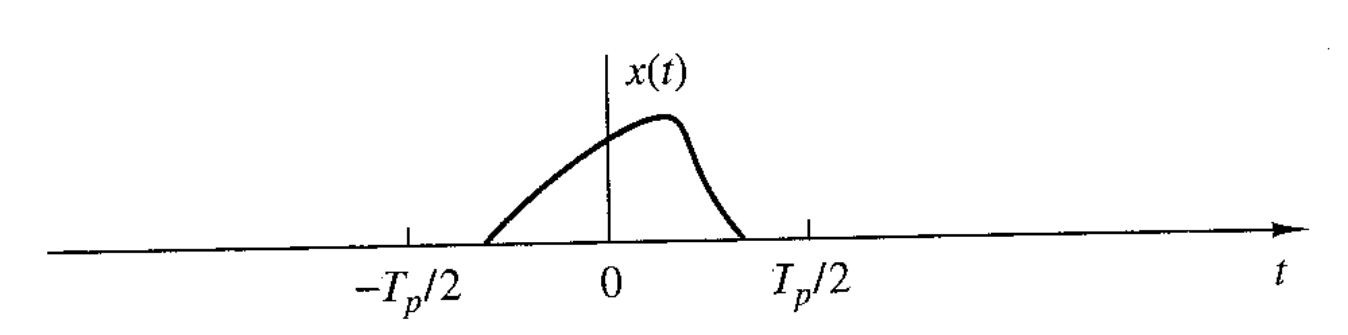
\includegraphics[width=1\linewidth, angle=-1]{imgs/proakis_aperiodic_1.png}
	\subcaption{Señal no periódicas.}
	\label{fig:senal_aperidica}
	\end{subfigure}

	\begin{subfigure}[b]{\columnwidth}
	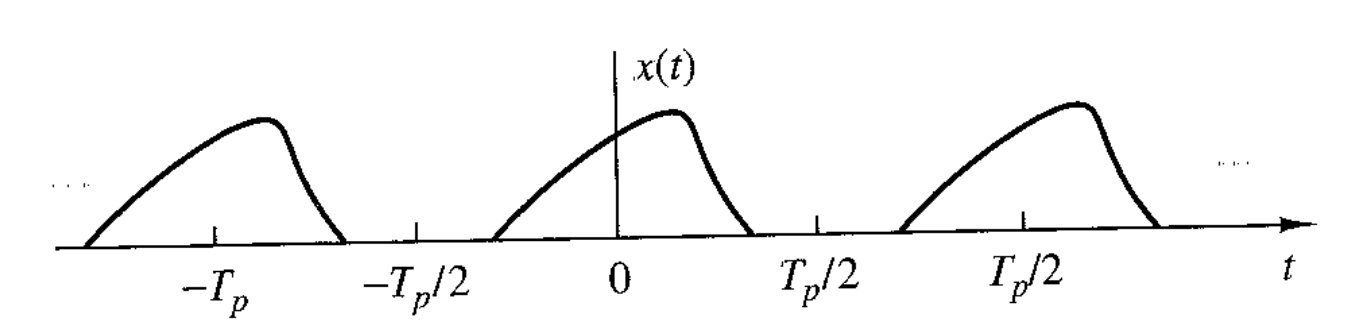
\includegraphics[width=1\linewidth, angle=-1]{imgs/proakis_aperiodic_2.png}
	\subcaption{Señal periódicas construida repitiendo (a).}
	\label{fig:senal_aperidocia_repetida}
	\end{subfigure}

\caption{Ejemplo de señal no periódicas\cite{proakis}.}
\label{fig:p4_both}
\end{figure}

El resultado de aplicar la transformada de Fourier a un función $f(x)$, cuyo dominio puede estan en el tiempo o espacio, es una función $\mathcal{F}(k)$, cuyo dominio se encuentra en el espacio de la frecuencia. En \ref{eq:ft} y \ref{eq:fti} se presenta las expresiones para el cálculo de la transformada de Fourier de una función y la de su inversa.

\begin{align}
	\mathcal{X}(F) &= \int_{-\infty}^{\infty} f(x) e^{-2\pi i F x} dt \label{eq:ft}\\
	x(t) &= \int_{-\infty}^{\infty} \mathcal{X}(F) e^{ 2\pi i F x} dF \label{eq:fti}
\end{align}

En general en la literatura es común encontrar \ref{eq:ft} y \ref{eq:fti} expresadas en funcion de la frecuencia angular $\omega = 2\pi F$.

\begin{align}
	\mathcal{X}(\omega) &= \int_{-\infty}^{\infty} f(x) e^{-i \omega x} dt \label{eq:ft}\\
	x(t) &= \frac{1}{2\pi} \int_{-\infty}^{\infty} \mathcal{X}(F) e^{i \omega x} d\omega \label{eq:fti}
\end{align}

\subsection{Series de Fourier - Señales Discretas}

De igual forma que una señal continua, una señal discreta $x(n)$ periódica con periodo $N$ tiene una representación en series de Fourier. La expasion en Series de Fourier se encuentra dada por \ref{eq:dfs}, mientras que el calculo de los coeficientes de la serie se realiza utilzando \ref{eq:dfs_coeffs}.

\begin{align}
	x(n) &= \sum_(k=0)^{N-1} c_k e^{\frac{i 2 \pi n}{N} k } \label{eq:dfs} \\
	c_k &= \frac{1}{N} \sum_(n=0)^{N-1} x(n) c_k e^{\frac{-i 2 \pi k}{N} n} \label{eq:dfs_coeffs}
\end{align}


\subsection{Transformada de Fourier - Señales Discretas}

De igual forma que en la señales continuas, es posible calcular la transformada de Fourier de una señal discreta. En \ref{eq:dft}  y  \ref{eq:dfti} se presentan la fórmulas para la Transforma de Fourier Discreta (DFT) y su inversa.

\begin{align}
	X(k) &= \sum_{n=0}^{N-1} x(n) e ^{-i \frac{2\pi}{N} k n } \label{eq:dft} \\
	x(n) &= \sum_{k=0}^{N-1} X(k) e ^{ i \frac{2\pi}{N} k n } \label{eq:dfti}
\end{align}

\subsection{Aplicación DFT en imagenes}

Dado que las imagenes son señales discretas en dos dimensiones para obtener su transformada de Fourier, basta con aplicarla en cada una de las dimensiones.

\begin{align}
	X(k,l) &= \sum_{i=0}^{N-1} \sum_{j=0}^{N-1} x(i,j) e ^ {-i \frac{2\pi}{N} (ki +lj)} \label{eq:dft2} \\
	X(i,j) &= \frac{1}{N^2} \sum_{k=0}^{N-1} \sum_{l=0}^{N-1} X(k,l) e ^ {i \frac{2\pi}{N} (ki +lj)} \label{eq:dft2}
\end{align}



%%%%%%%%%%%%%%%%%%%%%%%%%%%%%%%%%%%%%%%%%%%%%%%%%%%%%%%%%%%%%%%%%%%%%%%%%%%%%%%%
% Bibliography
\nocite{*}
\bibliographystyle{IEEEtran}
\bibliography{bibliography}


\end{document}



%\begin{lstlisting}[language=bash]
%  $ wget http://tex.stackexchange.com
%\end{lstlisting}

%\begin{table} \caption{A Simple Example Table} \label{table_example}
%  \begin{center}
%    \begin{tabular}{c c}
%      \hline
%      \bfseries First & \bfseries Next\\ \hline\hline
%      1.0 & 2.0 \\
%      \hline
%    \end{tabular}
%  \end{center}
%\end{table}


%\begin{lstlisting}[float=tbh!, caption={Magnitud de la respuesta en frecuencia del filtro IIR},label={cod:mag resp frec %IIR}]
%mag=20*log10(abs(H));
%\end{lstlisting}